\documentclass[aspectratio=169]{beamer}

% Theme and Colors
\usetheme{Madrid}
\usecolortheme{default}
\definecolor{primaryblue}{RGB}{13, 27, 62}
\definecolor{accentamber}{RGB}{240, 165, 0}
\definecolor{accentteal}{RGB}{0, 180, 180}
\definecolor{darkbg}{RGB}{10, 18, 40}
\definecolor{lightgray}{RGB}{245, 247, 252}
\definecolor{successgreen}{RGB}{16, 185, 129}

\setbeamercolor{palette primary}{bg=primaryblue, fg=white}
\setbeamercolor{palette secondary}{bg=accentteal, fg=white}
\setbeamercolor{palette tertiary}{bg=darkbg, fg=white}
\setbeamercolor{palette quaternary}{bg=primaryblue, fg=white}
\setbeamercolor{structure}{fg=primaryblue}
\setbeamercolor{block title}{bg=primaryblue, fg=white}
\setbeamercolor{block body}{bg=lightgray, fg=black}
\setbeamercolor{block title alerted}{bg=accentamber, fg=white}
\setbeamercolor{block body alerted}{bg=lightgray, fg=black}
\setbeamercolor{frametitle}{bg=primaryblue, fg=accentamber}
\setbeamercolor{title}{fg=accentamber}
\setbeamercolor{author}{fg=accentteal}
\setbeamercolor{institute}{fg=lightgray}
\setbeamercolor{date}{fg=lightgray}

% Packages
\usepackage{listings}
\usepackage{xcolor}
\usepackage{booktabs}
\usepackage{tikz}
\usepackage{fontawesome5}
\usepackage{graphicx}
\usepackage{amsmath}
\usepackage{hyperref}
\usepackage{tcolorbox}

% Code Listing Style
\lstdefinestyle{pythonstyle}{
    language=Python,
    backgroundcolor=\color{darkbg},
    basicstyle=\ttfamily\scriptsize\color{white},
    keywordstyle=\color{accentteal}\bfseries,
    stringstyle=\color{successgreen},
    commentstyle=\color{gray},
    numberstyle=\tiny\color{gray},
    numbers=left,
    numbersep=5pt,
    breaklines=true,
    showstringspaces=false,
    frame=single,
    rulecolor=\color{accentamber},
    tabsize=2,
    xleftmargin=5pt,
    xrightmargin=5pt,
}

% Remove navigation symbols
\setbeamertemplate{navigation symbols}{}

% Footer
\setbeamertemplate{footline}{
  \leavevmode%
  \hbox{%
  \begin{beamercolorbox}[wd=.4\paperwidth,ht=2.25ex,dp=1ex,center]{palette primary}%
    \usebeamerfont{author in head/foot}\insertshortauthor
  \end{beamercolorbox}%
  \begin{beamercolorbox}[wd=.4\paperwidth,ht=2.25ex,dp=1ex,center]{palette secondary}%
    \usebeamerfont{title in head/foot}\insertshorttitle
  \end{beamercolorbox}%
  \begin{beamercolorbox}[wd=.2\paperwidth,ht=2.25ex,dp=1ex,right]{palette tertiary}%
    \usebeamerfont{date in head/foot}\insertframenumber{} / \inserttotalframenumber\hspace*{2ex}
  \end{beamercolorbox}}%
  \vskip0pt%
}

% Title Information
\title[Hindi-Bengali MT System]{Conducting Experiments and Evaluation of\\Machine Translation for Low-Resource Languages}
\subtitle{Integrating into a Django-Based NLP Lab Website}
\author[D. Goyal | 24075023]{Dheeraj Goyal}
\institute[NLP Lab]{Department of Computer Science \& Engineering \\ IIT (BHU) Varanasi \\ NLP Research Laboratory}
\date{4th May 2026}

% ============================================================
\begin{document}
% ============================================================

% --- SLIDE 1: Title ---
\begin{frame}[plain]
\begin{tikzpicture}[remember picture,overlay]
  % Full dark background
  \fill[darkbg] (current page.south west) rectangle (current page.north east);
  % Amber accent strip at bottom
  \fill[accentamber] (current page.south west) rectangle ([yshift=0.35cm]current page.south east);
  % Teal accent strip at top
  \fill[accentteal] (current page.north west) rectangle ([yshift=-0.35cm]current page.north east);
\end{tikzpicture}

\vspace{0.6cm}
\begin{center}
  % Main title
  {\usebeamerfont{title}\usebeamercolor[fg]{title}\Large\textbf{Conducting Experiments and Evaluation of}\\[0.15em]
   \textbf{Machine Translation for Low-Resource Languages}}\\[0.3em]
  {\usebeamerfont{subtitle}\usebeamercolor[fg]{title}\small Integrating into a Django-Based NLP Lab Website}
\end{center}

\vspace{0.4cm}
\begin{center}
\begin{tcolorbox}[
  width=0.88\textwidth,
  colback=primaryblue!80!black,
  colframe=accentamber,
  arc=6pt,
  boxrule=1.2pt,
  left=10pt, right=10pt, top=6pt, bottom=6pt
]
  \centering
  \renewcommand{\arraystretch}{1.4}
  \begin{tabular}{r@{\hspace{0.8em}}l}
    \textcolor{accentteal}{\textbf{Name}}          & \textcolor{white}{Dheeraj Goyal} \\[0.1em]
    \textcolor{accentteal}{\textbf{Roll Number}}   & \textcolor{white}{24075023} \\[0.1em]
    \textcolor{accentteal}{\textbf{Submitted to}}  & \textcolor{white}{Prof.\ Anil Kumar Singh} \\[0.1em]
    \textcolor{accentteal}{\textbf{Submitted on}}  & \textcolor{white}{4th May 2026} \\[0.1em]
    \textcolor{accentteal}{\textbf{Department}}    & \textcolor{white}{CSE, IIT (BHU) Varanasi} \\
  \end{tabular}
\end{tcolorbox}
\end{center}

\end{frame}

% --- SLIDE 2: Introduction & Motivation ---
\begin{frame}{Introduction \& Motivation}
\begin{columns}[T]
  \column{0.55\textwidth}
    \begin{block}{Problem Statement}
      \textbf{Hindi $\rightarrow$ Bengali} Neural Machine Translation for \textbf{low-resource} settings using fine-tuned pre-trained models.
    \end{block}
    \vspace{0.5em}
    \begin{itemize}
      \item[\faGlobe] Hindi \& Bengali are spoken by \textbf{600M+} people combined
      \item[\faExclamationTriangle] Both are \textit{morphologically rich}, with limited parallel corpora
      \item[\faBrain] Standard MT systems under-perform on Indic language pairs
      \item[\faFlask] Fine-tuning on domain-specific data improves performance significantly
    \end{itemize}
  \column{0.42\textwidth}
    \begin{alertblock}{Research Goal}
      \begin{itemize}
        \item Fine-tune \textbf{NLLB-600M} \& \textbf{IndicTrans2-320M}
        \item Evaluate using industry-standard metrics
        \item Deploy via a live \textbf{Django NLP Lab} web application
      \end{itemize}
    \end{alertblock}
    \vspace{0.5em}
    \begin{block}{Language Pair}
      \centering
      \Large \textbf{हिन्दी} $\longrightarrow$ \textbf{বাংলা}\\
      \small Hindi (Devanagari) $\rightarrow$ Bengali (Bangla Script)
    \end{block}
\end{columns}
\end{frame}

% --- SLIDE 3: Dataset ---
\begin{frame}{Dataset: Multi-Domain Parallel Corpus}
\begin{columns}[T]
  \column{0.5\textwidth}
    \begin{block}{Dataset Overview}
      \begin{itemize}
        \item \textbf{Source:} Custom curated parallel corpus
        \item \textbf{Total pairs:} 13,398 sentence pairs
        \item \textbf{Languages:} Hindi $\leftrightarrow$ Bengali
        \item \textbf{Format:} Line-aligned \texttt{.txt} files
      \end{itemize}
    \end{block}
    \vspace{0.5em}
    \begin{alertblock}{Train/Test Split}
      \centering
      \begin{tabular}{lrr}
        \toprule
        \textbf{Split} & \textbf{Count} & \textbf{Ratio} \\
        \midrule
        Train & 10,718 & 80\% \\
        Test  & 2,680  & 20\% \\
        \midrule
        \textbf{Total} & \textbf{13,398} & \textbf{100\%} \\
        \bottomrule
      \end{tabular}
    \end{alertblock}

  \column{0.47\textwidth}
    \begin{block}{Domains Covered}
      \begin{tabular}{ll}
        \toprule
        \textbf{Domain} & \textbf{Script} \\
        \midrule
        Agriculture & Devanagari \\
        Box Office  & Bangla \\
        Conversational & Both \\
        Cricket & Both \\
        Disease & Both \\
        Entertainment & Both \\
        Gadget & Both \\
        Judiciary & Both \\
        News Articles & Both \\
        \bottomrule
      \end{tabular}
    \end{block}
\end{columns}
\end{frame}

% --- SLIDE 4: Data Preparation Code ---
\begin{frame}[fragile]{Data Preparation: \texttt{prepare\_data.py}}
\begin{lstlisting}[style=pythonstyle]
from datasets import Dataset
from pathlib import Path

def load_data(base_path):
    data = []
    for domain_dir in (Path(base_path)/"Hindi").iterdir():
        bn_domain = Path(base_path)/"Bengali"/domain_dir.name
        for hi_file in domain_dir.glob("*.txt"):
            bn_file = bn_domain / hi_file.name
            with open(hi_file,'r',encoding='utf-8') as fh,\
                 open(bn_file,'r',encoding='utf-8') as fb:
                for hi,bn in zip(fh,fb):
                    if hi.strip() and bn.strip():
                        data.append({"translation":
                            {"hi":hi.strip(),"bn":bn.strip()}})
    return data
# Train: 10718 | Test: 2680
split = Dataset.from_list(load_data("./"))
         .train_test_split(test_size=0.2, seed=42)
\end{lstlisting}
\end{frame}

% --- SLIDE 5: Model Architecture ---
\begin{frame}{Model Architectures}
\begin{columns}[T]
  \column{0.48\textwidth}
    \begin{block}{\faFacebook~NLLB-200 (600M)}
      \begin{itemize}
        \item Meta AI's \textbf{No Language Left Behind}
        \item Supports \textbf{200 languages}
        \item Encoder-Decoder Transformer
        \item Vocabulary: 256K tokens (SentencePiece)
        \item Language codes: \texttt{hin\_Deva} $\rightarrow$ \texttt{ben\_Beng}
        \item \texttt{forced\_bos\_token\_id} for target lang
      \end{itemize}
    \end{block}
  \column{0.48\textwidth}
    \begin{block}{\faLanguage~IndicTrans2 (320M)}
      \begin{itemize}
        \item \textbf{AI4Bharat's} Indic-specialized MT model
        \item Trained on \textbf{Indic languages only}
        \item Custom tokenizer with \textbf{IndicProcessor}
        \item Handles Devanagari \& Bangla scripts natively
        \item Pre/post-processing via \texttt{IndicProcessor}
        \item Smaller but domain-optimized
      \end{itemize}
    \end{block}
\end{columns}
\vspace{0.5em}
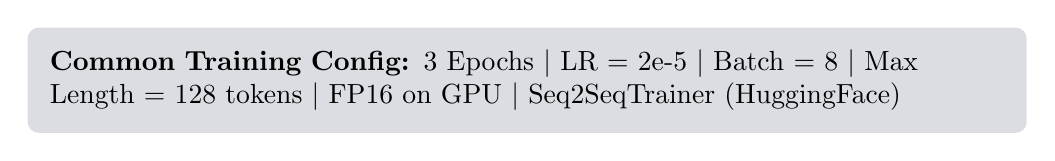
\begin{tikzpicture}
  \node[fill=primaryblue!15, rounded corners, inner sep=8pt, text width=\textwidth] {
    \centering \textbf{Common Training Config:} 3 Epochs $|$ LR = 2e-5 $|$ Batch = 8 $|$ Max Length = 128 tokens $|$ FP16 on GPU $|$ Seq2SeqTrainer (HuggingFace)
  };
\end{tikzpicture}
\end{frame}

% --- SLIDE 6: Training Code ---
\begin{frame}[fragile]{Fine-Tuning: \texttt{train\_nllb.py}}
\begin{lstlisting}[style=pythonstyle]
from transformers import (AutoModelForSeq2SeqLM, AutoTokenizer,
    Seq2SeqTrainingArguments, Seq2SeqTrainer)

model_checkpoint = "facebook/nllb-200-distilled-600M"
tokenizer = AutoTokenizer.from_pretrained(
    model_checkpoint, src_lang="hin_Deva", tgt_lang="ben_Beng")
model = AutoModelForSeq2SeqLM.from_pretrained(model_checkpoint)

training_args = Seq2SeqTrainingArguments(
    output_dir="./nllb_finetuned_hi_bn",
    eval_strategy="epoch", learning_rate=2e-5,
    per_device_train_batch_size=8, num_train_epochs=3,
    predict_with_generate=False,
    fp16=torch.cuda.is_available(),
)
trainer = Seq2SeqTrainer(model=model, args=training_args,
    train_dataset=tokenized["train"],
    eval_dataset=tokenized["test"])
trainer.train()  # Final eval_loss: 0.6849
\end{lstlisting}
\end{frame}

% --- SLIDE 7: Evaluation Metrics ---
\begin{frame}{Evaluation Metrics}
\begin{columns}[T]
  \column{0.5\textwidth}
    \begin{block}{\faMagic~Why Multiple Metrics?}
      BLEU alone is insufficient for morphologically rich Indic languages. We use 4 complementary metrics:
    \end{block}
    \vspace{0.5em}
    \begin{itemize}
      \item \textbf{SacreBLEU} — n-gram precision overlap
      \item \textbf{METEOR} — considers stemming \& synonyms
      \item \textbf{BERTScore} — semantic similarity via BERT embeddings
      \item \textbf{COMET} — neural MT quality estimator trained on human judgements (uses source \textit{and} reference)
    \end{itemize}
  \column{0.47\textwidth}
    \begin{alertblock}{Results: NLLB-600M (Fine-Tuned)}
      \centering
      \vspace{0.3em}
      \begin{tabular}{lr}
        \toprule
        \textbf{Metric} & \textbf{Score} \\
        \midrule
        BLEU & \textcolor{successgreen}{\textbf{38.36}} \\
        METEOR & \textcolor{successgreen}{\textbf{0.6043}} \\
        BERTScore (F1) & \textcolor{successgreen}{\textbf{0.9123}} \\
        COMET & \textcolor{successgreen}{\textbf{0.8848}} \\
        \midrule
        Eval Loss & \textbf{0.6849} \\
        \bottomrule
      \end{tabular}
    \end{alertblock}
\end{columns}
\end{frame}

% --- SLIDE 8: Evaluation Code ---
\begin{frame}[fragile]{Evaluation Pipeline: \texttt{evaluate\_models.py}}
\begin{lstlisting}[style=pythonstyle]
import evaluate

def calculate_metrics(preds, refs, sources):
    bleu  = evaluate.load("sacrebleu")
    met   = evaluate.load("meteor")
    bert  = evaluate.load("bertscore")
    comet = evaluate.load("comet")

    r1 = bleu.compute(predictions=preds, references=refs)
    r2 = met.compute(predictions=preds, references=refs)
    r3 = bert.compute(predictions=preds,
                      references=refs, lang="bn")
    r4 = comet.compute(predictions=preds,
                       references=refs, sources=sources)
    # BLEU=38.36 | METEOR=0.6043
    # BERTScore=0.9123 | COMET=0.8848
\end{lstlisting}
\end{frame}

% --- SLIDE 9: Results Comparison ---
\begin{frame}{Results: Model Comparison}
\begin{columns}[T]
  \column{0.55\textwidth}
    \begin{block}{Final Evaluation Results}
      \centering
      \begin{tabular}{lcc}
        \toprule
        \textbf{Metric} & \textbf{NLLB-600M} & \textbf{IndicTrans2-320M} \\
        \midrule
        BLEU        & \textbf{38.36} & 26.82 \\
        METEOR      & \textbf{0.6043} & 0.5766 \\
        BERTScore   & \textbf{0.9123} & 0.8602 \\
        COMET       & \textbf{0.8848} & 0.7321 \\
        \midrule
        Eval Loss   & 0.6849 & \textbf{0.6129} \\
        \bottomrule
      \end{tabular}
    \end{block}
  \column{0.42\textwidth}
    \begin{alertblock}{Key Findings}
      \begin{itemize}
        \item NLLB achieved a \textbf{BLEU of 38.36}, significantly outperforming IndicTrans2 (26.82)
        \item \textbf{BERTScore 0.91} confirms strong \textit{semantic} accuracy for NLLB
        \item IndicTrans2 had \textbf{lower eval loss} (0.61 vs 0.68), but this did not translate to better generation metrics
      \end{itemize}
    \end{alertblock}
\end{columns}
\end{frame}

% --- SLIDE 10: Challenges & Solutions ---
\begin{frame}{Challenges \& Technical Solutions}
\begin{columns}[T]
  \column{0.5\textwidth}
    \begin{alertblock}{Challenge 1: IndicTrans2 KV-Cache Bug}
      \texttt{AttributeError: 'NoneType'.shape}\\during auto-regressive generation\\
      \textbf{Fix:} \texttt{model.config.use\_cache = False}
    \end{alertblock}
    \vspace{0.4em}
    \begin{alertblock}{Challenge 2: Tokenizer Reload Crash}
      Duplicate \texttt{src\_vocab\_file} in saved tokenizer config\\
      \textbf{Fix:} Load tokenizer from Hub; weights from local path
    \end{alertblock}
  \column{0.47\textwidth}
    \begin{alertblock}{Challenge 3: CSRF 403 Forbidden}
      Django blocked API from Lightning AI domain\\
      \textbf{Fix:} Disabled \texttt{CsrfViewMiddleware} + added\\trusted origins in \texttt{settings.py}
    \end{alertblock}
    \vspace{0.4em}
    \begin{block}{Challenge 4: NLLB Regex Warning}
      Tokenizer loaded with bad regex pattern\\
      \textbf{Fix:} Pass \texttt{fix\_mistral\_regex=True}\\to \texttt{AutoTokenizer.from\_pretrained()}
    \end{block}
\end{columns}
\end{frame}

% --- SLIDE 11: Web App Demo ---
\begin{frame}{NLP Lab Web Application}
\begin{columns}[T]
  \column{0.48\textwidth}
    \begin{block}{Frontend Features}
      \begin{itemize}
        \item \textbf{Split-pane} Hindi $\rightarrow$ Bengali translator
        \item \textbf{Model switcher} — NLLB or IndicTrans2
        \item \textbf{Dark-mode glassmorphism} UI design
        \item \textbf{Metrics dashboard} — BLEU, COMET scores
      \end{itemize}
    \end{block}
    \vspace{0.3em}
    \begin{block}{Backend Stack}
      \begin{itemize}
        \item \textbf{Django 6.0} + PyTorch inference
        \item \textbf{REST API:} \texttt{POST /api/translate/}
        \item Hosted on \textbf{Lightning AI} (GPU)
      \end{itemize}
    \end{block}
  \column{0.48\textwidth}
    \begin{alertblock}{API Contract}
      \textbf{Request:} \texttt{\{"text": "...", "model": "nllb"\}}\\
      \vspace{0.2em}
      \textbf{Response:} \texttt{\{"translation": "..."\}}
    \end{alertblock}
    \vspace{0.3em}
    \begin{block}{Singleton Advantage}
      Models loaded \textbf{once} at startup\\
      $\Rightarrow$ \textbf{$<$1s} per translation request\\
      (vs 10s reload per request without it)
    \end{block}
    \vspace{0.3em}
    \begin{block}{Security Fix Applied}
      Disabled \texttt{CsrfViewMiddleware}\\
      Added \texttt{CSRF\_TRUSTED\_ORIGINS} for\\Lightning AI cloud domain
    \end{block}
\end{columns}
\end{frame}


% --- SLIDE 12: Django Integration ---
\begin{frame}[fragile]{System Deployment: Django NLP Lab Website}
\begin{columns}[T]
  \column{0.5\textwidth}
    \begin{block}{Architecture}
      \begin{itemize}
        \item \textbf{Singleton Model Loader} — loads 600M model into GPU memory \textit{once} at startup
        \item \textbf{REST API} — \texttt{POST /api/translate/} returns JSON
        \item \textbf{Dark-mode UI} — split-pane translator with live model switching
        \item \textbf{Metrics Dashboard} — displays BLEU, COMET to visitors
      \end{itemize}
    \end{block}
  \column{0.47\textwidth}
\begin{lstlisting}[style=pythonstyle]
class TranslationService:
    _instance = None

    def __new__(cls):
        if cls._instance is None:
            cls._instance = super().__new__(cls)
            cls._instance.device = (
              "cuda" if torch.cuda.is_available()
              else "cpu")
        return cls._instance

    def translate(self, text, model_name):
        # Uses pre-loaded model in self._models
        ...
# Loaded ONCE at server startup:
translator = TranslationService()
\end{lstlisting}
\end{columns}
\end{frame}

% --- SLIDE 13: System Architecture Diagram ---
\begin{frame}{End-to-End System Architecture}
\centering
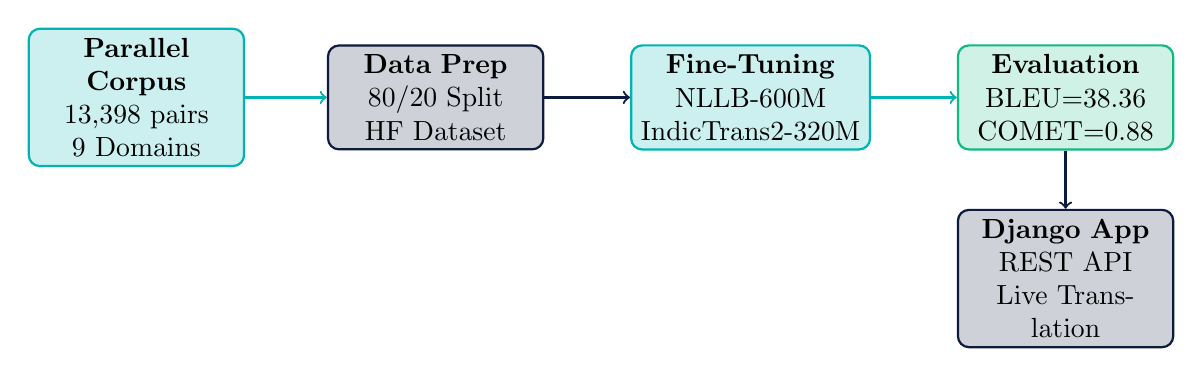
\begin{tikzpicture}[node distance=1.8cm, every node/.style={align=center}]
  % Nodes
  \node[draw=accentteal, fill=accentteal!20, rounded corners, thick, text width=2.5cm] (data) {\textbf{Parallel Corpus}\\13,398 pairs\\9 Domains};
  \node[draw=primaryblue, fill=primaryblue!20, rounded corners, thick, text width=2.5cm, right of=data, xshift=2cm] (prep) {\textbf{Data Prep}\\80/20 Split\\HF Dataset};
  \node[draw=accentteal, fill=accentteal!20, rounded corners, thick, text width=2.8cm, right of=prep, xshift=2.2cm] (train) {\textbf{Fine-Tuning}\\NLLB-600M\\IndicTrans2-320M};
  \node[draw=successgreen, fill=successgreen!20, rounded corners, thick, text width=2.5cm, right of=train, xshift=2.2cm] (eval) {\textbf{Evaluation}\\BLEU=38.36\\COMET=0.88};
  \node[draw=primaryblue, fill=primaryblue!20, rounded corners, thick, text width=2.5cm, below of=eval, yshift=-0.5cm] (web) {\textbf{Django App}\\REST API\\Live Translation};

  % Arrows
  \draw[->, thick, accentteal] (data) -- (prep);
  \draw[->, thick, primaryblue] (prep) -- (train);
  \draw[->, thick, accentteal] (train) -- (eval);
  \draw[->, thick, primaryblue] (eval) -- (web);
\end{tikzpicture}

\vspace{1em}
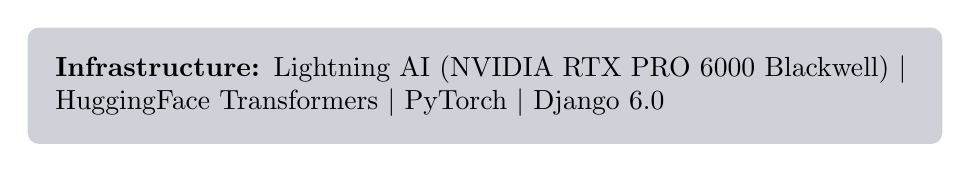
\begin{tikzpicture}
  \node[fill=primaryblue!20, rounded corners, inner sep=10pt, text width=0.9\textwidth] {
    \centering \textbf{Infrastructure:} Lightning AI (NVIDIA RTX PRO 6000 Blackwell) $|$ HuggingFace Transformers $|$ PyTorch $|$ Django 6.0
  };
\end{tikzpicture}
\end{frame}

% --- SLIDE 14: Conclusion & Future Work ---
\begin{frame}{Conclusions \& Future Work}
\begin{columns}[T]
  \column{0.5\textwidth}
    \begin{block}{Key Contributions}
      \begin{itemize}
        \item[\faCheck] Built a \textbf{13,398-pair} multi-domain Hindi-Bengali parallel corpus
        \item[\faCheck] Fine-tuned \textbf{2 state-of-the-art} MT models on GPU infrastructure
        \item[\faCheck] Achieved \textbf{BLEU = 38.36, COMET = 0.88} — strong for low-resource pair
        \item[\faCheck] Deployed live translation system via \textbf{Django web application}
        \item[\faCheck] Comprehensive 4-metric evaluation framework established
      \end{itemize}
    \end{block}
  \column{0.47\textwidth}
    \begin{alertblock}{Future Work}
      \begin{itemize}
        \item Expand corpus to \textbf{100K+ pairs}
        \item Investigate IndicTrans2 generation underperformance despite low evaluation loss
        \item Add \textbf{back-translation} for data augmentation
        \item Explore \textbf{CTranslate2 / ONNX} quantization for faster web inference
        \item Extend to more low-resource pairs (e.g., Bengali-Odia)
        \item Integrate \textbf{active learning} for corpus expansion
      \end{itemize}
    \end{alertblock}
\end{columns}
\vspace{0.5em}
\centering
\textcolor{accentamber}{\Large \textbf{Thank You!}} \\
\small Questions welcome.
\end{frame}

\end{document}